\section{Sơ đồ Lược đồ Logic (Logical Schema Diagram)}

Lược đồ dưới đây tương ứng với tập phụ thuộc hàm đã xét ở mục chuẩn hóa. Các ràng buộc miền giá trị và duy nhất bổ sung được trình bày ở từ điển dữ liệu.

Đặc biệt, hệ thống tồn tại mối kết hợp Nhiều - Nhiều (M:N) giữa \texttt{CUSTOMER} và \texttt{MERCHANT}. Mối kết hợp này đã được phân rã thành hai mối quan hệ 1-N thông qua thực thể trung gian (Associative Entity) là bảng \texttt{CREDIT}.

Dưới đây là Sơ đồ Logic thể hiện trực quan cấu trúc các bảng, tập hợp đầy đủ các thuộc tính, khóa chính (Primary Key - PK) và các mối quan hệ khóa ngoại (Foreign Key - FK) kèm bản số (1-N) liên kết giữa các bảng.

\begin{figure}[H]
    \centering
    \resizebox{\textwidth}{!}{ % Co theo chieu rong trang
    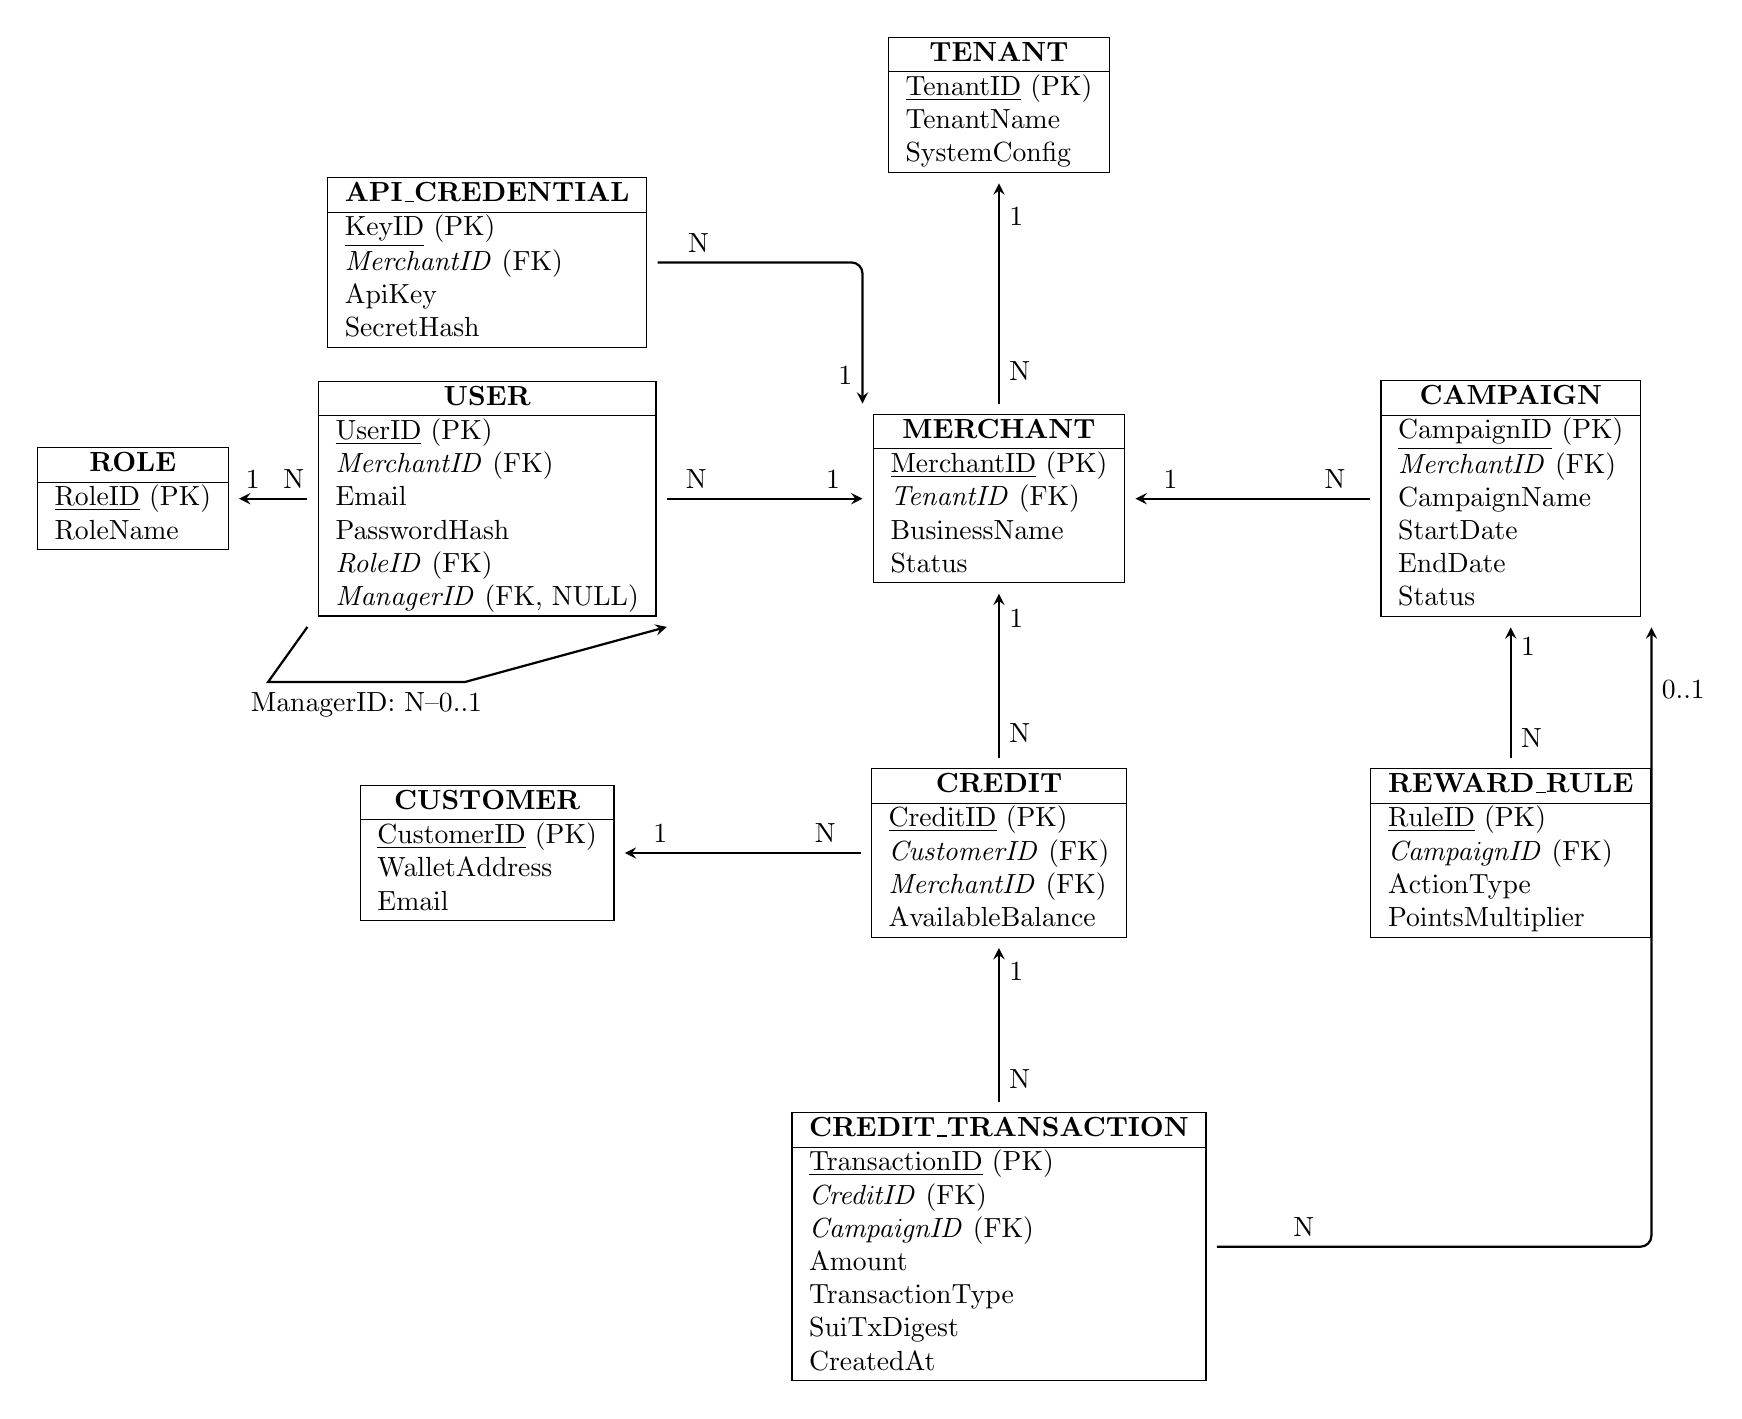
\begin{tikzpicture}[>=stealth, thick]

        % Bảng TENANT
        \node (tenant) at (0, 6.5) {
            \begin{tabular}{|l|}
            \hline
            \multicolumn{1}{|c|}{\textbf{TENANT}} \\ \hline
            \underline{TenantID} (PK) \\
            TenantName \\
            SystemConfig \\ \hline
            \end{tabular}
        };

        % Bảng MERCHANT
        \node (merchant) at (0, 1.5) {
            \begin{tabular}{|l|}
            \hline
            \multicolumn{1}{|c|}{\textbf{MERCHANT}} \\ \hline
            \underline{MerchantID} (PK) \\
            \textit{TenantID} (FK) \\
            BusinessName \\
            Status \\ \hline
            \end{tabular}
        };

        % Bảng API_CREDENTIAL (Đã bổ sung)
        \node (api) at (-6.5, 4.5) {
            \begin{tabular}{|l|}
            \hline
            \multicolumn{1}{|c|}{\textbf{API\_CREDENTIAL}} \\ \hline
            \underline{KeyID} (PK) \\
            \textit{MerchantID} (FK) \\
            ApiKey \\
            SecretHash \\ \hline
            \end{tabular}
        };

        % Bảng USER
        \node (user) at (-6.5, 1.5) {
            \begin{tabular}{|l|}
            \hline
            \multicolumn{1}{|c|}{\textbf{USER}} \\ \hline
            \underline{UserID} (PK) \\
            \textit{MerchantID} (FK) \\
            Email \\
            PasswordHash \\
            \textit{RoleID} (FK) \\
            \textit{ManagerID} (FK, NULL) \\ \hline
            \end{tabular}
        };

        % Bang ROLE va quan he quan ly tu tham chieu
        \node (role) at (-11, 1.5) {
            \begin{tabular}{|l|}
            \hline
            \multicolumn{1}{|c|}{\textbf{ROLE}} \\ \hline
            \underline{RoleID} (PK) \\
            RoleName \\ \hline
            \end{tabular}
        };
        \draw[->] (user.west) -- node[pos=0.2, above] {N} node[pos=0.8, above] {1} (role.east);
        \draw[->] (user.south west) -- ++(-0.5,-0.7) -- ++(2.5,0)
            node[midway, below] {ManagerID: N--0..1} -- (user.south east);

        % Bảng CAMPAIGN
        \node (campaign) at (6.5, 1.5) {
            \begin{tabular}{|l|}
            \hline
            \multicolumn{1}{|c|}{\textbf{CAMPAIGN}} \\ \hline
            \underline{CampaignID} (PK) \\
            \textit{MerchantID} (FK) \\
            CampaignName \\
            StartDate \\
            EndDate \\
            Status \\ \hline
            \end{tabular}
        };

        % Bảng CUSTOMER
        \node (customer) at (-6.5, -3) {
            \begin{tabular}{|l|}
            \hline
            \multicolumn{1}{|c|}{\textbf{CUSTOMER}} \\ \hline
            \underline{CustomerID} (PK) \\
            WalletAddress \\
            Email \\ \hline
            \end{tabular}
        };

        % Bảng CREDIT (Bảng trung gian giải quyết quan hệ N-N)
        \node (credit) at (0, -3) {
            \begin{tabular}{|l|}
            \hline
            \multicolumn{1}{|c|}{\textbf{CREDIT}} \\ \hline
            \underline{CreditID} (PK) \\
            \textit{CustomerID} (FK) \\
            \textit{MerchantID} (FK) \\
            AvailableBalance \\ \hline
            \end{tabular}
        };

        % Bảng REWARD_RULE
        \node (rule) at (6.5, -3) {
            \begin{tabular}{|l|}
            \hline
            \multicolumn{1}{|c|}{\textbf{REWARD\_RULE}} \\ \hline
            \underline{RuleID} (PK) \\
            \textit{CampaignID} (FK) \\
            ActionType \\
            PointsMultiplier \\ \hline
            \end{tabular}
        };

        % Bảng CREDIT_TRANSACTION
        \node (transaction) at (0, -8) {
            \begin{tabular}{|l|}
            \hline
            \multicolumn{1}{|c|}{\textbf{CREDIT\_TRANSACTION}} \\ \hline
            \underline{TransactionID} (PK) \\
            \textit{CreditID} (FK) \\
            \textit{CampaignID} (FK) \\
            Amount \\
            TransactionType \\
            SuiTxDigest \\
            CreatedAt \\ \hline
            \end{tabular}
        };

        % ========================================================
        % VẼ DÂY NỐI CÓ GẮN NHÃN BẢN SỐ (1 và N)
        % ========================================================
        
        % MERCHANT -> TENANT
        \draw[->] (merchant.north) -- node[pos=0.15, right] {N} node[pos=0.85, right] {1} (tenant.south);
        
        % API -> MERCHANT (Dây gấp khúc)
        \draw[->, rounded corners] (api.east) -| node[pos=0.1, above] {N} node[pos=0.9, left] {1} (merchant.north west);
        
        % USER -> MERCHANT
        \draw[->] (user.east) -- node[pos=0.15, above] {N} node[pos=0.85, above] {1} (merchant.west);
        
        % CAMPAIGN -> MERCHANT
        \draw[->] (campaign.west) -- node[pos=0.15, above] {N} node[pos=0.85, above] {1} (merchant.east);
        
        % CREDIT -> MERCHANT
        \draw[->] (credit.north) -- node[pos=0.15, right] {N} node[pos=0.85, right] {1} (merchant.south);
        
        % CREDIT -> CUSTOMER
        \draw[->] (credit.west) -- node[pos=0.15, above] {N} node[pos=0.85, above] {1} (customer.east);
        
        % REWARD_RULE -> CAMPAIGN
        \draw[->] (rule.north) -- node[pos=0.15, right] {N} node[pos=0.85, right] {1} (campaign.south);
        
        % TRANSACTION -> CREDIT
        \draw[->] (transaction.north) -- node[pos=0.15, right] {N} node[pos=0.85, right] {1} (credit.south);
        
        % TRANSACTION -> CAMPAIGN (Dây gấp khúc vòng lên)
        \draw[->, rounded corners] (transaction.east) -| node[pos=0.1, above] {N} node[pos=0.95, right] {0..1} (campaign.south east);

    \end{tikzpicture}
    }
    \caption{Sơ đồ Lược đồ Logic chi tiết hệ thống OctaPoint CaaS}
    \label{fig:sodo_logic_tikz}
\end{figure}

\textit{Ghi chú:} Sơ đồ thể hiện rõ việc phân rã mối kết hợp N-N giữa Khách hàng và Doanh nghiệp thông qua thực thể trung gian \texttt{CREDIT}. Các đường liên kết chỉ hướng tham chiếu từ Khóa ngoại (nhánh N) trỏ tới Khóa chính (nhánh 1), đảm bảo chặt chẽ ràng buộc toàn vẹn tham chiếu.
Mỗi cặp (CustomerID, MerchantID) ở CREDIT có tối đa một bản ghi. Nhãn N chỉ số lượng tối đa ở phía tham chiếu; RoleID bắt buộc, ManagerID và CampaignID của giao dịch tùy chọn.
